\chapter{Implementierung}
\label{ch:implementierung}

\section{Netzwerk- und Speicherstruktur der Container-Umgebung}
Die gesamte Umgebung wird durch eine \texttt{docker-compose.yml} orchestriert. Orchestrierung bedeutet die automatische Vernetzung und Verwaltung der erstellten Container, sodass diese als zusammenhängendes System funktionieren \parencite{AWS}. In der \texttt{docker-compose.yml} wird das interne Netzwerk \texttt{matomo\textunderscore network} erstellt, über welches die Container miteinander kommunizieren. Zusätzlich werden persistente Volumes definiert, um sicherzustellen, dass die Daten über Neustarts der Container hinweg erhalten bleiben. Das Volume \texttt{matomo} speichert sämtliche Konfigurationsdateien des Webanalysetools. Somit können die Matomo Einstellungen, beispielsweise für den Datenschutz persistent gespeichert werden. Die Datenbank, welche alle erfassten Trackingdaten enthält wird in dem Volume \texttt{db} gespeichert. Für die Visualisierung speichert das Volume \texttt{grafana-storage} die Konfigurationen von Grafana, sowie die erstellten Dashboards und Panels. Das Bildungsportal wird als externes Volume \texttt{portal} aus dem Projektverzeichnis eingebunden.

\section{Reverse Proxy und Dienstweiterleitung}
Der Reverse Proxy (Nginx) wird als Zugangspunkt für die Dienste verwendet. Die Konfigurationsdatei \texttt{reverse\textunderscore proxy.conf} dient dazu, die externen Anfragen an die Dienste weiterzuleiten. Somit werden die Website, Matomo und Grafana unter separaten Pfaden erreichbar gemacht: 

\textbf{Matomo} wird über den Reverse Proxy unter \texttt{/matomo} bereitgestellt. Da das verwendete Matomo-Docker-Image \texttt{/matomo:5.2.2-fpm-alpine} keinen eigenen Webserver mitbringt, wird in der \texttt{docker-compose.yml} ein zusätzlicher Nginx-Webserver (\texttt{matomo\textunderscore web}) definiert. Dieser empfängt Anfragen vom Reverse Proxy und leitet sie über das FastCGI-Protokoll an PHP-FPM (FastCGI Process Manager) weiter, da Matomo auf PHP basiert. PHP-FPM ist ein Prozessmanager für PHP \parencite{PHPFPM}, welcher von Matomo verwendet wird. Da Nginx als Reverse Proxy keine PHP-Skripte selbst verarbeiten kann, sondern diese an eine externe Instanz übergeben muss \parencite{NginxReverseProxy}, ist dieser zusätzliche Webserver erforderlich. Dieser benötigt ebenfalls eine Konfig-Datei (\texttt{matomo.conf}), die sicherstellt, dass alle Anfragen korrekt verarbeitet und an PHP-FPM übergeben werden. Während die \texttt{reverse\textunderscore proxy.conf} externe Anfragen an \texttt{/matomo} an \texttt{matomo\textunderscore web} weiterleitet, definiert die \texttt{matomo.conf}, wie diese innerhalb des Containers verarbeitet werden. Der \texttt{matomo\textunderscore web}-Container besitzt kein öffentliches Port-Mapping und ist ausschließlich über den Reverse Proxy erreichbar.

\textbf{Grafana} wird unter \texttt{/grafana} bereitgestellt. Im Gegensatz zu Matomo benötigt Grafana keinen separaten Webserver, da es über einen integrierten Webserver verfügt. Dadurch kann Grafana direkt über den Reverse Proxy erreichbar gemacht werden.

\textbf{Die Website} wird unter \texttt{/evaschiffmann} bereitgestellt. Sie wird ebenfalls wie Matomo über einen Nginx-Webserver ausgeliefert, der ausschließlich für die Bereitstellung der Inhalte zuständig ist. Genauso wie \texttt{matomo\textunderscore web} besitzt auch dieser Webserver kein öffentliches Port-Mapping, sodass die Website nur über den Reverse Proxy aufgerufen werden kann. Dieser nimmt die Anfragen entgegen und leitet sie an den internen Nginx-Container weiter, welcher die Website ausliefert.

\begin{figure}[H]
    \centering
    \begin{minipage}{\textwidth}
        \lstinputlisting[
            caption=Docker Container zur Bereitstellung des Nginx Reverse Proxy, 
            label={lst:reverseproxy},
            language={}, 
            style=yaml
        ]{listings/reverse-proxy.yml}
    \end{minipage}
\end{figure}

Das Listing~\ref{lst:reverseproxy} zeigt die Definition des Reverse Proxy in der \texttt{docker-compose.yml}. Die einzelnen Komponenten werden anhand der Kommentare beschrieben. Um die Dienste über HTTPS verfügbar zu machen, wurde für die Testumgebung auf localhost ein selbst signiertest Zertifikat hierfür erstellt und eingebunden. Dies ist in Zeile acht zu erkennen. In Zeile zehn wird das Volume für Matomo gemountet, sprich eingebunden. Dies dient zur Bereitstellung von statischen Inhalten wie HTML oder Javascript. PHP-Anfragen werden wie bereits erwähnt an \texttt{matomo\textunderscore web} weitergeleitet.

\section{Integration der Webanalyse mit Matomo}
Nachdem die Webserver aufgesetzt wurden und die \texttt{docker-compose.yml} definiert wurde, ist Matomo in der lokalen Umgebung über \textit{https://localhost/matomo} verfügbar und die Einrichtung kann erfolgen. Die Einrichtung besteht im wesentlichen aus fünf Schritten. Zunächst wird ein System Check durchgeführt, bei dem überprüft wird, ob die Serverumgebung die Anforderungen für den Betrieb von Matomo erfüllt. Hierbei wird unter anderem geprüft, ob eine kompatible PHP-Version verwendet wird oder auch ob Matomo auf die notwendigen Verzeichnisse zugreifen kann und Schreibrechte für diese besitzt. Nach dem erfolgreichen System Check kann die Datenbankverbindung eingerichtet werden und ein Hauptadministrator angelegt werden. 

\begin{figure}[H]
    \centering
    \begin{minipage}{0.49\textwidth}
        \centering
        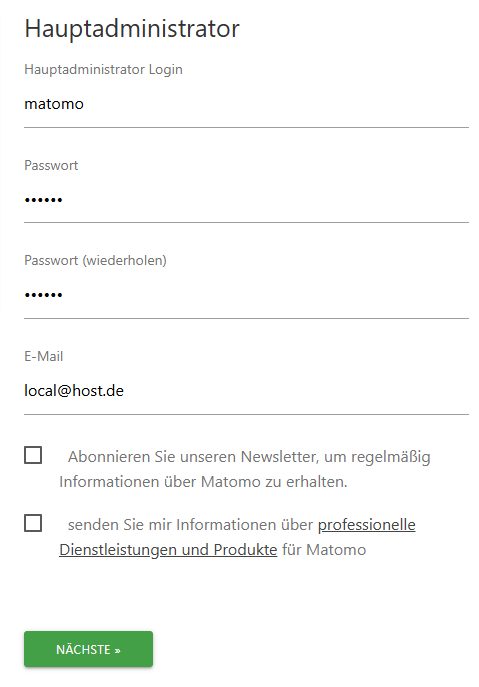
\includegraphics[width=\linewidth, keepaspectratio]{images/haupadministrator.png}
        \caption{Anlegen des Kontos für den Hauptadministrator in Matomo.}
        \label{fig:hauptadministrator}
    \end{minipage}
    \hfill
    \begin{minipage}{0.49\textwidth}
        \centering
        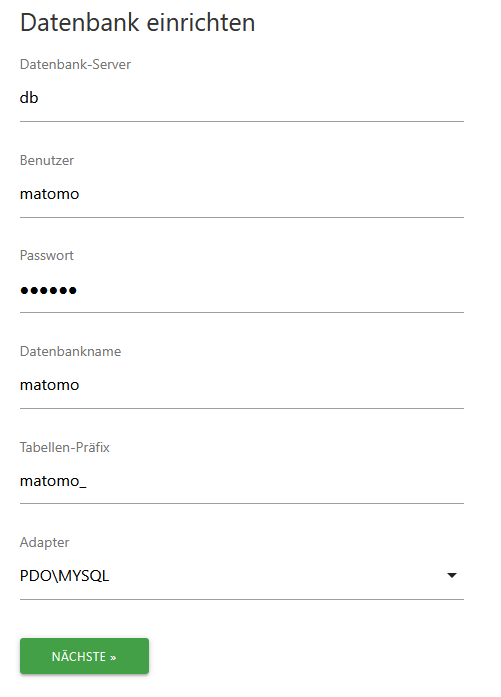
\includegraphics[width=\linewidth, keepaspectratio]{images/setup-datenbank.png}
        \caption{Einrichtung der Datenbankverbindung in Matomo.}
        \label{fig:setup-datenbank}
    \end{minipage}
\end{figure}

In Abbildung~\ref{fig:hauptadministrator} ist zu sehen wie das Konto erstellt wird. In Abbildung~\ref{fig:setup-datenbank} wird gezeigt, wie die Datenbankverbindung zu MariaDB hergestellt wird. Die Zugangsdaten für den Hauptadministrator, sowie den Datenbanknutzer sind in der Datei \texttt{db.env} gespeichert. Für die Datenbank wird der Container \texttt{db} verwendet. In diesem Container wird dafür gesorgt, dass folgendes Skript eingebunden wird: 

\begin{figure}[H]
    \centering
    \begin{minipage}{\textwidth}
        \lstinputlisting[
            caption=SQL-Skript für die Erstellung eines Nutzer mit read-only Rechten., 
            label={lst:readonly},
            language=sql
        ]{listings/create-read-only-user.sql}
    \end{minipage}
\end{figure}

Das in Listing~\ref{lst:readonly} zu sehende Skript erstellt einen neuen Datenbanknutzer, welcher ausschließlich Leseberechtigung auf die Datenbanktabellen von Matomo besitzt. Dieser Datenbanknutzer soll später für die Anbindung an Grafana verwendet werden, um sicherzustellen, dass über Grafana keine Daten manipuliert werden können. Im vorletzten Schritt der Einrichtung wird die Website konfiguriert, welche von Matomo getrackt werden soll: 

\begin{figure}[H]
    \centering
    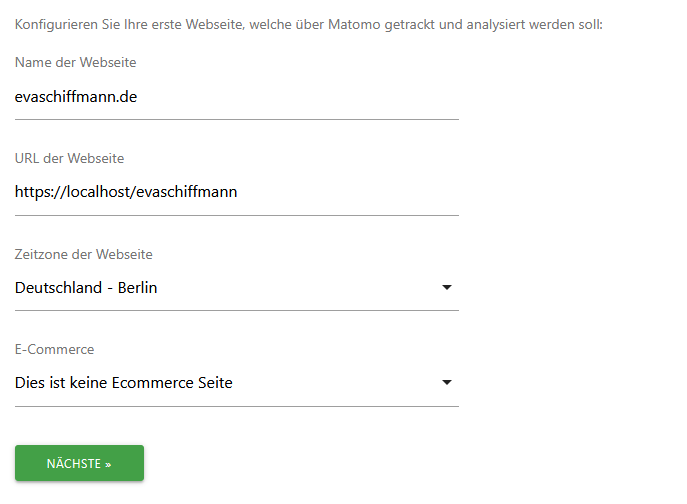
\includegraphics[width=\textwidth, keepaspectratio]{images/website-hinzufuegen.png}
    \caption{Hinzufügen der Website für das Matomo-Tracking}
    \label{fig:website-hinzufuegen}
\end{figure}

Wie in Abbildung~\ref{fig:website-hinzufuegen} zu erkennen, erhält die Website ebenfalls einen Namen in Matomo. Somit kann in Matomo direkt erkannt werden, welche Website gerade getrackt wird. 

Im letzten Schritt der Matomo-Einrichtung wird das Page-Tag von Matomo generiert. Um dieses nutzbar zu machen wird es anschließend vor dem \texttt{</body>}-Tag jeder Seite integriert, um sicherzustellen, dass der Inhalt der Seite geladen wurde. Da die gespiegelte Website sehr viele HTML-Dateien beinhaltet wurde hierfür ein Python Skript (\texttt{insert\allowbreak-scripts.py}) geschrieben, welches dafür sorgt, dass das Page-Tag in alle HTML-Dateien per Skript-Tag eingefügt wird. Das Skript selbst befindet sich in der Datei \texttt{tracking.js}. 


\section{Matomo datenschutzkonform konfigurieren}
Damit sichergestellt wird, dass Nutzer nicht über ihre IP-Adressen identifiziert werden können, wird in Matomo innerhalb der Einstellungen zur Privatsphäre eine IP-Anonoymisierung konfiguriert. Hierbei werden die letzten 2 bytes der IP-Adresse anonymisiert. 

Um sicherzustellen, dass Nutzer nur dann getrackt werden, wenn diese ihre Zustimmung erteilen, werden Opt-In- und Opt-Out-Mechanismen für die Einwilligung und den Widerruf der Tracking-Berechtigungen implementiert. Hierfür wurde im Page-Tag die in Listing~\ref{lst:require-consent} zu sehende Zeile hinzugefügt: 

\begin{figure}[H]
    \centering
    \begin{minipage}{\textwidth}
        \lstinputlisting[
            caption=Funktion zur Überprüfung der Nutzereinwilligung für das Tracking in Matomo., 
            label={lst:require-consent},
        ]{listings/require-consent.js}
    \end{minipage}
\end{figure}

Hierdurch verhindert Matomo, dass Tracking-Daten automatisch erfasst werden, solange keine Einwilligung vorliegt. Erst wenn der Nutzer aktiv zustimmt, wird das Tracking aktiviert \parencite{MatomoConsent}.

Die Zustimmung, also das Opt-In, erfolgt über das Cookie-Banner. Wenn hierbei auf \glqq Ok\grqq{} geklickt wird, wird der in Listing~\ref{lst:remember-consent-given} zu sehende Programmcode ausgeführt:

\begin{figure}[H]
    \centering
    \begin{minipage}{\textwidth}
        \lstinputlisting[
            caption=Programmcode zum setzen der Zustimmung für das Tracking in Matomo., 
            label={lst:remember-consent-given},
        ]{listings/remember-consent-given.js}
    \end{minipage}
\end{figure}

Sobald hierbei der Klick auf \glqq Ok\grqq{} erfolgt ist, wird die Funktion \texttt{rememberConsentGiven} ausgeführt. Diese Funktion sorgt dafür, dass ein Cookie Namens \glqq consent\grqq{} im Browser des Nutzers gesetzt wird \parencite{MatomoConsent}. So lange dieser Cookie existiert hat Matomo die Erlaubnis Daten zu sammeln \parencite{MatomoConsent}. Zusätzlich wird der Einwilligungsstatus im lokalen Speicher des Browsers (\texttt{localStorage}) gespeichert.

Die Speicherung zusätzlich im lokalen Speicher des Browsers ist notwendig, da dieser Status in der Datei \texttt{withdraw-consent.js} verwendet wird. Die Logik dieser Datei ist in Listing~\ref{lst:withdraw-consent} zu erkennen: 

\begin{figure}[H]
    \centering
    \begin{minipage}{\textwidth}
        \lstinputlisting[
            caption=Programmcode zur Speicherung und Verwaltung der Tracking-Einwilligung mittels Local Storage.,
            label={lst:withdraw-consent},
        ]{listings/withdraw-consent.js}
    \end{minipage}
\end{figure}

In Zeile zwei wird als erstes geprüft, ob der Consent für das Tracking erteilt wurde. Auf der Datenschutzseite wurde ein Button für das Widerufen und die Zustimmung zum Tracking hinzugefügt. In den Zeilen sieben bis zehn wird der Button-Text entsprechend des aktuellen Tracking-Status gesetzt. Ist das Tracking bereits aktiv, wird der Text \glqq Tracking deaktivieren\grqq{} angezeigt, andernfalls erscheint \glqq Tracking erlauben\grqq{}. Die Zeilen 14 bis 28 enhalten die Logik um die Zustimmung oder Ablehnung den Trackings zu setzen. Hierbei wird jeweils eine Meldung an den Nutzer gegeben, dass die Aktion erfolgreich war. Im lokalen Speicher des Browsers wird ebenfalls der Status zur Zustimmung gespeichert. Die Zustimmung über den Button erfolgt ebenfalls wie bei dem Cookie-Banner über \texttt{rememberConsentGiven}. Für das Widerrufen der Berechtigung wird die Funktion \texttt{forgetConsentGiven} verwendet, welche dafür sorgt, dass der gesetzte \glqq consent\grqq{}-Cookie gelöscht wird \parencite{MatomoConsent}.

\section{Einrichtung der Datenquelle in Grafana}
Grafana ist in der lokalen Umgebung unter \textit{https://localhost/grafana} verfügbar. Wird diese URL aufgerufen, erscheint zunächst der Login-Screen zur Anmeldung. Nach erfolgter Anmeldung wird die Grafana Oberfläche geladen. Um nun Analysedaten von Matomo zu erhalten muss zunächst eine Datenquelle eingerichtet werden. Da direkt auf Daten aus der Matomo Datenbank zugegriffen werden soll, wird hierfür die Grafana Datenquelle \glqq MySQL\grqq{} verwendet.

\begin{figure}[H]
    \centering
    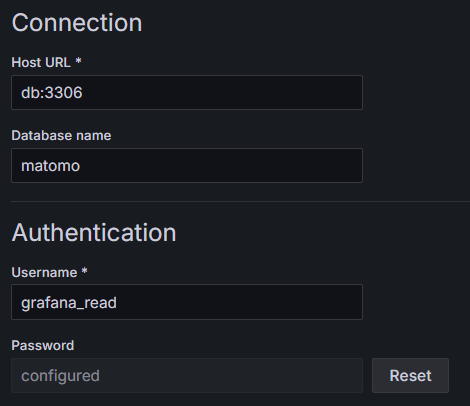
\includegraphics[width=0.6\textwidth, keepaspectratio]{images/datasource.png}
    \caption{Einrichtung der Datenquelle in Grafana über das MySQL-Plugin.}
    \label{fig:datasource}
\end{figure}

In der Abbildung~\ref{fig:datasource} ist zu sehen, dass der Datenbank-Container \texttt{db} mit dem Standardport für MySQL, bzw. MariaDB als Host URL gesetzt wurde. Dies ist möglich, da Grafana und Matomo über das gemeinsame Netzwerk \texttt{matomo\textunderscore network} innerhalb der Container-Umgebung kommunizieren können. Somit kann direkt der Containername, anstatt einer URL verwendet werden. Ebenfalls zu erkennen ist, dass der zuvor erstellte Datenbanknutzer, welcher ausschließlich Leseberechtigungen auf die Matomo Datenbank besitzt verwendet wird, um Daten abzurufen. Wenn nun Panels zur Visualisierung der Analysewerte erstellt werden, kann diese Datenquelle ausgewählt werden um über den read-only Nutzer der Datenbank SQL-Abfragen an diese zu erstellen.

\section{Umsetzung der Filtermöglichkeiten in Grafana}
Um die zeitliche Filterung der erhaltenen Daten einheitlich über alle Pannels hinweg zu ermöglichen wird der Grafana Time Picker verwendet. Damit dieser funktionsfähig ist, müssen die über den Time Picker eingestellten Werte in die SQL-Abfrage integriert werden. Hierfür werden die Grafana-Variablen \texttt{\$\{\_\_from\}} und \texttt{\$\{\_\_to\}} genutzt, welche das Start- und Enddatum der vom Nutzer gewählten Zeitspanne enthalten \parencite{GrafanaTimePickerVariables}. 

\begin{figure}[H]
    \centering
    \begin{minipage}{\textwidth}
        \lstinputlisting[
            caption=Zeitliche Filterung der Besuchsdaten in Grafana mittels \texttt{visit\_first\_action\_time} und den Time-Picker-Variablen \texttt{\$\{\_\_from\}} und \texttt{\$\{\_\_to\}}.,
            label={lst:from-to},
            language=sql
        ]{listings/from-to.sql}
    \end{minipage}
\end{figure}

In dem Listing~\ref{lst:from-to} werden die Grafana Variablen für die Zeitbegrenzung verwendet. Da der Time Picker nur Unix Zeitstempel zurückgibt, müssen diese in das passende Datumsformat der Datenbank umgewandelt werden. Hierfür bietet MySQL die Funktion \texttt{FROM\textunderscore UNIXTIME} \parencite{MySQLUnixtime}. Die Tabelle \texttt{log\textunderscore visit} wird für die Zeitbegrenzung verwendet und speichert die einzelnen Nutzersitzungen \parencite{MatomoDBSchema}. In dieser Tabelle befindet sich die Spalte \texttt{visit\textunderscore first \textunderscore action\textunderscore time}, welche den Zeitpunkt der ersten Aktion einer Sitzung speichert \parencite{MatomoDBSchema}. Da jeder Eintrag eine eigenständige Sitzung darstellt, können darüber Sitzungen gefiltert werden, die im gewählten Zeitraum stattgefunden haben.

Um die Filterung der Werte für die einzelnen Unterseiten zu realisieren, wird in Grafana die Variable \texttt{\$Seite} definiert. Diese hat als Werte die Titel der Unterseiten des Bildungsportals, also beispielsweise \glqq Zum Tagebuch\grqq{} oder \glqq Schülerin\grqq{}. Die Variable kann ebenfalls den Wert \glqq Übersicht\grqq{} haben. Wenn dieser Wert ausgewählt wird werden die angzeigten Daten nicht auf eine bestimmte Unterseite begrenzt, sondern beziehen sich auf das gesamte Bildungsportal. Ebenso kann für die Variable der Wert \glqq Alle Tagebuchseiten\grqq{} ausgewählt werden. Hierbei werden alle Tagebuchseiten zusammengefasst um eine Übersicht, über die allgemeine Nutzung des Tagebuchs zu zeigen. Nachdem die Variable definiert wurde, wird diese in der Dashboardansicht sichtbar und über ein Drop-Down Menü können die einzelnen Werte der Variable ausgewählt werden.

\begin{figure}[H]
    \centering
    \begin{minipage}{\textwidth}
        \lstinputlisting[
            caption=SQL-Abfrage zur Filterung der Besuche basierend auf der ausgewählten Unterseite oder den Tagebuchseiten.,
            label={lst:seite},
            language=sql
        ]{listings/seite.sql}
    \end{minipage}
\end{figure}

Das Listing~\ref{lst:seite} zeigt, auf welche Art und Weise die Variable \texttt{\$Seite} in den SQL-Abfragen verwendet wird. Über diese Query werden alle Besuche auf der Website ausgegeben, entweder ungefiltert, für eine Unterseite oder für alle Tagebuchseiten. Über den ersten \texttt{JOIN} in Zeile fünf werden die Sitzungen mit den zugehörigen Aktionen, also unter anderem Seitenaufrufen, verknüpft. Da die Seitentitel allerdings in der Tabelle \texttt{log\textunderscore action} gespeichert werden, wird hierfür ein weiterer \texttt{JOIN} benötigt. In der {\texttt{WHERE}-Klausel} wird zuletzt der Wert der Variable geprüft. Ist dieser \glqq Übersicht\grqq{}, wird keine Filterung vorgenommen und alle Besuche werden angezeigt. Wird eine Unterseite ausgewählt, werden nur die Besuche auf dieser Seite ausgegeben. Für die Tagebuchseiten wurde ein regulärer Ausdruck verwendet, da die Titel für die Tagebuchseiten immer den Bezeichner \glqq Blatt\grqq{} mit der entsprechenden Nummer besitzen.

Die Variable \texttt{\$Seite} wird in diesen Metriken verwendet: 
\begin{itemize}
    \item Anzahl der Besuche
    \item Anzahl der wiederkehrenden Besucher
    \item Anteil der wiederkehrenden Besucher
    \item Anzahl der einmaligen Besucher
    \item Ranking der am häufigsten aufgeklappten Überschriften
    \item Verweildauer
\end{itemize}

Um die Sortierrichtung der Tabellen, sowie des Balkendiagramms umzukehren, wird eine Variable namens \texttt{\$Sort} definiert. Diese Variable hat die Werte \textit{ASC} (aufsteigend) und \textit{DESC} (absteigend).

\begin{figure}[H]
    \centering
    \begin{minipage}{\textwidth}
        \lstinputlisting[
            caption=SQL-Abfrage zur Identifikation von Traffic-Quellen sowie zur Erfassung der Seitenaufrufe und Absprungraten über diese.,
            label={lst:referer-ranking},
            language=sql
        ]{listings/referer-ranking.sql}
    \end{minipage}
\end{figure}

Die Query aus Listing~\ref{lst:referer-ranking} zeigt wie die Variable \texttt{\$Sort} verwendet wird. Je nach Auswahl wird der Wert in die {\texttt{ORDER BY}-Klausel} geschrieben. Der \texttt{referer\textunderscore type} wird in der Datenbank als Zahlenwert gespeichert, wobei jede Zahl einen Quelle angibt \parencite{MatomoDBSchema}. Wenn der Zugriff nicht über einen Referer erfolgt, ist der \texttt{referer\textunderscore type} gleich \glqq 1\grqq{}. Dieser Wert wird somit ausgeschlossen. Matomo speichert in der Datenbank ebenfalls die Aktionen, welche auf der Website ausgeführt wurden, nachdem der Besucher über einen Referer auf die Seite gelangt ist. Wenn nur eine Aktion ausgeführt wurde, so wird der \texttt{bounce\textunderscore count} gesetzt. Dieser Zähler erhöht sich um eins, wenn Besucher nur eine Aktion ausführen, wenn diese über eine externe Quelle auf das Bildungsportal gelangt sind. Die Gruppierung erfolgt über die \texttt{referer\textunderscore url}, sodass die Besuche und Absprünge für jede URL angezeigt werden. 

Die Variable \texttt{\$Sort} wird in diesen Metriken verwendet: 
\begin{itemize}
    \item Ranking der Referer Seiten
    \item Seitenaufrufe nach Häufigkeit
    \item Ranking der am häufigsten aufgeklappten Überschriften
\end{itemize}

\section{Erstellung der Panels in Grafana}
In diesem Abschnitt wird beschrieben, wie sich die einzelnen Abfragen zu den Analysewerten zusammensetzen und wie die Panels für die Visualisierung konfiguriert werden, um die in Abschnitt~\ref{sec:Visualisierungsmethoden} beschriebenen Visualisierungsformen für die entsprechenden Analysewerte zu verwenden. 

\subsection{Ranking der Referer Seiten}
Die Abfrage für diese Metrik, ist in Listing~\ref{lst:referer-ranking} zu sehen und wurde bereits erläutert. In den Panel-Einstellungen wird als Darstellungsform die Tabelle ausgewählt. Über die Einstellung \glqq Show table header\grqq{} wird eingestellt, dass die in der SQL-Abfrage definierten Namen für die Tabellen im Panel angezeigt werden. Außerdem wurde für die Größe der Tabelle die \glqq Cell Height\grqq{}
(Zeilenhöhe) auf \glqq Medium\grqq{} gesetzt. Eine kleinere Zeilenhöhe würde die Übersichtlichkeit beeinträchtigen, während eine größere dazu führen würde, dass weniger Werte auf einen Blick erfassbar sind. Der Hintergrund für die Spalten \texttt{Besuche} und \texttt{Bounce\textunderscore Count} wurde mit dem Lila-Farbton des Bildungsportals versehen, während die Spalte \texttt{Referer} den Gelbton des Bildungsportals erhalten hat.

\subsection{Verteilung der Traffic Quellen}
Für die Verteilung der Traffic Quellen wird in Grafana ein Pie-Chart-Panel erstellt um die Daten in einem Kreisdiagramm zu visualisieren. Hierbei ist es wichtig, dass die Einstellung \texttt{Show} auf \glqq All values\grqq{} gesetzt wird. Andernfalls würde die Gesamtzahl der Traffic-Quellen angezeigt werden. Grafana bietet die Darstellungsformen \texttt{Pie} und \texttt{Donut}, für das Pie-Chart-Panel. Hierbei bietet die \texttt{Pie}-Option die Größere Fläche für die Darstellung der Prozentwerte, weshalb diese Option verwendet wird. Ein Tooltip wird integriert, der beim Überfahren der einzelnen Bereiche des Kreisdiagramms mit der Maus den jeweiligen Prozentwert anzeigt. Ebenfalls gibt es eine Legende, welche die einzelnen Werte, mit den entsprechenden Farben, sowie Prozentwerten darstellt.

Für die Datenbankabfrage wird die Tabelle \texttt{log\textunderscore visit} verwendet, in welcher die Referer-Informationen gespeichert werden. Die in Lisiting~\ref{lst:referer-ranking} aufgezeigten \texttt{referer\textunderscore types}, kommen für diese Metrik ebenfalls zum Einsatz. Zusätzlich wird der Wert \glqq 1\grqq{} mit aufgenommen, um den Prozentsatz der Nutzer, welche direkt auf die Website über die Eingabe der URL oder auch über ein Lesezeichen gelangt sind zu berücksichtigen. Damit im Kreisdiagramm die richtigen Werte für die verschiedenen Quellen angezeigt werden, müssen diese entsprechend dem \texttt{referer\textunderscore type} gruppiert werden.

\subsection{Seitenaufrufe nach Häufigkeit}
Für diese Metriken wird ein Bar-Chart-Panel verwendet. Hierfür bietet Grafana umfangreiche Konfigurationsmöglichkeiten: 

\begin{figure}[H]
    \centering
    \begin{minipage}{0.49\textwidth}
        \centering
        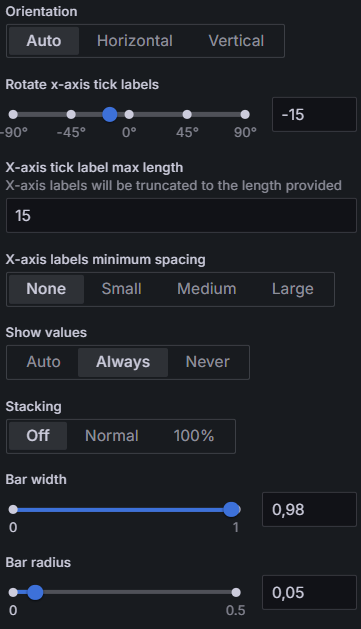
\includegraphics[width=\linewidth, keepaspectratio]{images/orientation.png}
        \caption{Anpassung der Balkendiagramm-Ausrichtung, Balkenbreite und Beschriftungen in Grafana.}
        \label{fig:orientation}
    \end{minipage}
    \hfill
    \begin{minipage}{0.49\textwidth}
        \centering
        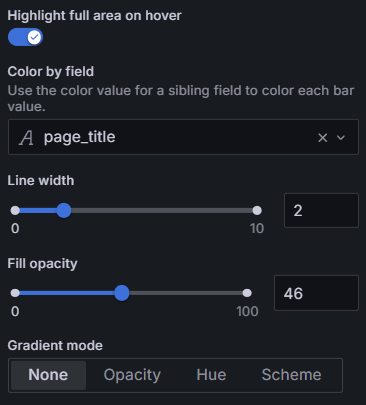
\includegraphics[width=\linewidth, keepaspectratio]{images/highlight.png}
        \caption{Einstellungen zur Hervorhebung und Farbgebung im Balkendiagramm in Grafana.}
        \label{fig:highlight}
    \end{minipage}
\end{figure}

Wie in Abbildung~\ref{fig:orientation} zu sehen ist, wird der Winkel der X-Achsen-Beschriftungen leicht angepasst, um die Lesbarkeit der Seitentitel zu verbessern und ein Überlappen der Texte zu vermeiden. Zusätzlich wird die maximale Zeichenlänge der X-Achsen-Beschriftungen auf \glqq 15\grqq{} begrenzt, sodass lange Titel gekürzt werden. Die Ausrichtung des Diagramms kann zwischen horizontal und vertikal gewechselt werden, wobei die aktuelle Einstellung \glqq Auto\grqq{} einer horizontalen Darstellung entspricht. Zudem wird die Balkenbreite und der Balkenradius angepasst, um ein abgerundetes Design zu erzeugen. Durch die aktivierte Option \texttt{Show values} wird sichergestellt, dass die Zahlenwerte direkt auf den Balken angezeigt werden, ohne das diese nochmal separat angeklickt werden müssen.

In Abbildung~\ref{fig:highlight} sind die Einstellungen für die optische Darstellung der Balken zu sehen. Hier wird festgelegt, dass beim Überfahren eines Balkens mit der Maus der gesamte Bereich farblich markiert wird. Die Farbgebung der Balken richtet sich nach dem Feld \texttt{page\textunderscore title}, um eine visuelle Unterscheidung zwischen den einzelnen Seitentiteln zu ermöglichen. Unterseiten erhalten jeweils eine eigene Farbe, wobei für alle Tagebuchseiten die selbe Farbe verwendet wird. Das ist ebenfalls der Fall für die Unterseiten von \glqq Wer War Eva Schiffmann\grqq{} und \glqq Themen\grqq{}. Diese Entscheidung wurde getroffen, da ansonsten mit verschiedenen Farbtönen einer Farbe gearbeitet werden müsste und somit die Unterscheidung zwischen den Seiten schwerer fällt. Darüber hinaus wird die Linienbreite reduziert und die Transparenz der Balkenfüllung angepasst, um das Diagramm optisch ansprechender zu machen.

\begin{figure}[H]
    \centering
    \begin{minipage}{\textwidth}
        \lstinputlisting[
            caption=SQL-Abfrage zur für die Metrik \glqq Seitenaufrufe nach Häufigkeit\grqq{},
            label={lst:seitenaufrufe},
            language=sql
        ]{listings/seitenaufrufe.sql}
    \end{minipage}
\end{figure}

Das Listing~\ref{lst:seitenaufrufe} zeigt die SQL-Abfrage zur Ermittlung der zehn meist- oder wenigstbesuchten Unterseiten. Über einen \texttt{JOIN} wird die Tabelle \texttt{log\textunderscore link\textunderscore visit\textunderscore action} mit \texttt{log\textunderscore action} verknüpft, um die zugehörigen Seitentitel abzurufen. Ein weiterer \texttt{JOIN} mit der Tabelle \texttt{log\textunderscore visit} verknüpft die Aktionen mit den jeweiligen Besuchssitzungen.

Zusätzlich wird über eine \texttt{CASE}-Anweisung geprüft, ob es sich bei einer Seite um eine Tagebuchseite handelt. In diesem Fall wird mithilfe eines regulären Ausdrucks der Titel standardisiert, sodass alle Tagebuchseiten unter einer gemeinsamen Bezeichnung zusammengefasst werden. Die Abfrage zählt die Seitenaufrufe, sortiert sie nach Häufigkeit und gibt die zehn meist- oder wenigstbesuchten Seiten zurück.

\subsection{Ranking der am häufigsten aufgeklappten Überschriften}
Diese Metrik verwendet ebenfalls eine Tabelle für die Visualisierung. Wie bei der Tabelle \glqq Ranking der Referer Seiten\grqq{} werden die Farben des Bildungsportals für die Hintergründe der Spalten gesetzt. Die Spalte \glqq Anzahl\grqq{} hat den Lila-Farbton und der Hintergrund der Spalte \glqq Titel\grqq{} ist gelb. Der \glqq Titel\grqq{} gibt an, um welche Überschrift es sich handelt und die \glqq Anzahl\grqq{} zeigt, wie oft die Überschrift aufgeklappt wurde. Die Panel-Einstellungen werden ebenfalls identisch zu Metrik \glqq Ranking der Referer Seiten\grqq{} gesetzt, um für ein einheitliches Design zu sorgen. Da für das Aufklappen der Überschriften kein Page-View getriggert wird, muss um diese Metrik zu erfassen ein Event definiert werden. Dieses wird in Listing~\ref{lst:headingsevent} dargestellt:

\begin{figure}[H]
    \centering
    \begin{minipage}{\textwidth}
        \lstinputlisting[
            caption=Matomo-Event für die Erfassung der Interaktionen mit den Überschriften.,
            label={lst:headingsevent},
        ]{listings/headings-event.js}
    \end{minipage}
\end{figure}

In diesem Programmcode werden Events gesendet, sobald mit einer Überschrift auf der Website interagiert wird. Neben dem Event für das Aufklappen der Überschriften, wird noch ein Event für das Zuklappen benötigt. Die Differenz zwischen dem Aufklappen und Zuklappen wird genutzt, um zu bestimmen, wie lange der Text gelesen wurde. Die Kategorie des Events \texttt{expand} enhält außerdem den Titel der Überschrift. Für das \texttt{close}-Event wird der Titel nicht benötigt, da sich dieses immer auf die zuvor aufgeklappte Überschrift bezieht. Dies ist möglich, da Überschriften auf der Website automatisch zugeklappt werden, wenn eine weitere Überschrift aufgeklappt wird. Das Event \texttt{close} wird für diese Metrik zwar nicht benötigt, spielt aber für die Analyse einer Nutzersitzung eine Rolle.

Die Abfrage zu diesem Panel verwendet für die Events die Tabelle \texttt{log\textunderscore action}. Da für das „Ranking der am häufigsten aufgeklappten Überschriften“ nur das Event \texttt{expand} berücksichtigt wird, wird \texttt{log\textunderscore action} mehrfach per Self-Join eingebunden. Das ist notwendig, da Matomo Kategorie, Aktion und Label eines Events gemeinsam in dieser Tabelle speichert. Um alle drei Bestandteile getrennt auswerten zu können, muss die Tabelle mit unterschiedlichen Aliasen gejoint werden. Nur so lässt sich beispielsweise der Titel (Label) mit der Aktion \texttt{expand} korrekt verknüpfen. Die Tagebuchseiten enthalten ebenfalls jeweils drei Überschriften, welche für jede Seite gleich sind. Damit diese Überschriften in dem Panel ignoriert werden, wird die in Listing~\ref{lst:ignorieren} zu sehende Zeile in der Query ergänzt: 

\begin{figure}[H]
    \centering
    \begin{minipage}{\textwidth}
        \lstinputlisting[
            caption=Ausschnitt einer SQL-Abfrage\, um die Überschriften innerhalb der Tagebuchseiten zu ignorieren.,
            label={lst:ignorieren},
            language=sql
        ]{listings/ignore.sql}
    \end{minipage}
\end{figure}

\texttt{event\textunderscore label} ist ein Alias für die Tabelle \texttt{log\textunderscore action} und über das Attribut \texttt{name} wird der Titel der Überschrift gefiltert.

\subsection{Besuche, einmalige Besucher und wiederkehrende Besucher}
Zur Darstellung dieser drei Metriken wird ein einfaches statisches Panel verwendet und der Hintergrund wird auf den Gelbton des Bildungsportal gesetzt.

Die Abfrage für die Besuche ermittelt die Gesamtanzahl der Nutzer, die eine Seite des Bildungsportals besucht haben. Dafür wird die Tabelle \texttt{log\textunderscore action} mit \texttt{log\allowbreak\_link\allowbreak\_visit\allowbreak\_action} verknüpft. Die Anzahl der unterschiedlichen Visit-ID's in der Tabelle \texttt{log\textunderscore action} entspricht hierbei der Anzahl der Besuche. Die Tabelle \texttt{log\textunderscore link\textunderscore visit\textunderscore action} wird verwendet um die Anzahl der Besuche über die Variable \texttt{\$Seite} für eine Unterseite über den Titel zu filtern.

Die Query für die wiederkehrenden Besucher basiert auf derselben Tabellenstruktur, konzentriert sich aber auf Nutzer, welche die Website bereits zuvor besucht haben. Dazu wird \texttt{visitor\textunderscore returning = 1} als Bedingung gesetzt. Der Wert \glqq 1\grqq{} gibt an, dass der Besucher bereits zuvor auf der Website war. Die Zählung erfolgt, anders als bei der Metrik für die Besuche, über die Visitor-ID. Der Unterschied hierbei ist, dass nicht einzelne Sitzungen (Besuche) gezählt werden, sondern tatsächliche Besucher.

Die Metrik für die einmaligen Besucher identifiziert Nutzer, die exakt eine Session auf der Website hatten. Über eine Unterquery wird geprüft, welche Visitor-ID's nur genau einmal in der \texttt{log\textunderscore action}-Tabelle vorkommen, also nur eine einzelne Sitzung aufweisen. Das geschieht über die Filterung \texttt{HAVING COUNT(idvisit) = 1}. Die Seitenfilterung erfolgt auch hierbei genauso wie für die Besuche.

\subsection{Anteil der wiederkehrenden Besucher}
Der \glqq Anteil der wiederkehrenden Besucher\grqq{} wird über ein Gauge-Panel realisiert. Der Wert erhält außerdem die Maßeinheit \%. Es werden drei Grenzwerte (engl. Thresholds) definiert, um dabei zu helfen den angezeigten Wert auf den ersten Blick einzuordnen. Die Thresholds sind in Abbildung~\ref{fig:thresholds} zu sehen: 

\begin{figure}[H]
    \centering
    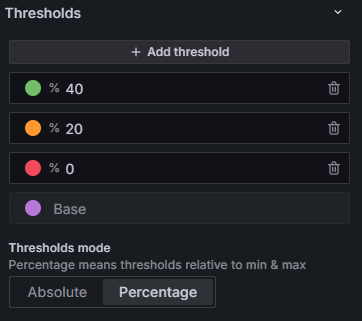
\includegraphics[width=0.6\textwidth, keepaspectratio]{images/thresholds.png}
    \caption{Grenzwerte für den \glqq Anteil der wiederkehrenden Besucher\grqq{}.}
    \label{fig:thresholds}
\end{figure}

In Abbildung~\ref{fig:thresholds} ist zu erkennen, dass wenn der Wert kleiner als 20 \% ist, die Farbe auf rot gesetzt wird. Zwischen 20 \% und 39 \% wird der Wert orange und ab 40 grün. Da es sich bei diesem Analysewert um ein Verhältnis handelt, muss der \texttt{Thresholds mode} entsprechend gesetzt werden, damit die Farben korrekt zugeordnet werden können. Damit diese Thresholds als Markierung an dem Panel angezeigt werden, wird zusätzlich die Option \texttt{Show threshold markers} aktiviert. Die Berechnung des Prozentwertes ist in Listing~\ref{lst:wiederkehrende-besucher} aufgezeigt:

\begin{figure}[H]
    \centering
    \begin{minipage}{\textwidth}
        \lstinputlisting[
            caption=Berechnung für den \glqq Anteil der wiederkehrenden Besucher\grqq{} in SQL.,
            label={lst:wiederkehrende-besucher},
            language=sql
        ]{listings/wiederkehrende-besucher.sql}
    \end{minipage}
\end{figure}

Der Dividend entspricht der Anzahl der wiederkehrenden Besucher, während der Divisor die Gesamtzahl aller Besuche darstellt.

\subsection{Gerätetypen}
Für die Aufteilung der Gerätetypen, wird ebenfalls wie für die \glqq Verteilung der Traffic Quellen\grqq{} ein Pie-Chart-Panel verwendet und in den Panel-Einstellungen genauso konfiguriert, um für ein konsistentes Design zu sorgen. Der einzige Unterschied ist, dass die Legende für diese Metrik aus Platzgründen rechts von dem Kreisdiagramm angezeigt wird.

\begin{figure}[H]
    \centering
    \begin{minipage}{\textwidth}
        \lstinputlisting[
            caption=Unterscheidung von Gerätetypen in Matomo.,
            label={lst:geraetetypen},
            language=sql
        ]{listings/geraetetypen.sql}
    \end{minipage}
\end{figure}

Der Ausschnitt der Query für die Zuordnung (engl. Mapping) der Werte für die Gerätetypen ist in Listing~\ref{lst:geraetetypen} aufgelistet. Der \texttt{config\textunderscore device\textunderscore type} wird ebenfalls wie der \texttt{referer\textunderscore type} als Zahlenwert in der Datenbank gespeichert \parencite{GithubDevices}. Für den Fall, dass ein Gerät verwendet wird, welches nicht explizit gemappt wurde, wird der Wert \glqq Unknown\grqq{} gesetzt. Der \texttt{config\textunderscore device\textunderscore type} ist ebenfalls in der Tabelle \texttt{log\textunderscore visit} zu finden. 

\subsection{Bounce Rate}
Die \glqq Bounce Rate\grqq{} wird in Prozent angegeben und beschreibt, wie viele Nutzer nur eine einzige Aktion auf der Website durchgeführt haben und diese anschließend direkt wieder verlassen haben \parencite[S.33]{Dykes2014}. Da es sich bei dieser Metrik um ein Verhältnis handelt wäre hierfür ein Gaug-Panel eine gute Wahl. Um das Dashboard jedoch übersichtlich zu halten und den Nutzer nicht mit zu vielen Gauge-Visualisierungen zu überfordern, wird die Bounce Rate stattdessen in einem Stat-Panel dargestellt. Der Hintergrund wird hierbei, ebenso wie bei den bereits erläuterten Stat-Panels auf den Gelbton des Bildungsportals gesetzt.

Für die Berechnung wird das Attribut \texttt{visit\textunderscore total\textunderscore actions} der Tabelle \texttt{log\textunderscore visit} verwendet. Der Dividend bildet sich aus allen \texttt{visit\textunderscore total\textunderscore actions} welche den Wert \glqq 1\grqq{} haben. Also aus allen Besuchen, in welchen nur eine Aktion erfolgt ist. Der Dividend ist die Anzahl aller Sitzungen.

\subsection{Verweildauer}
Für die Darstellung der Verweildauer wird ebenfalls ein Stat-Panel konfiguriert, da hierbei ein einzelner Zahlenwert zusammen mit der Einheit Minuten dargestellt wird. Auch hier wird der Gelbton des Bildungsportals als Hintergrundfarbe gesetzt.

Für diesen Analysewert kommen zwei Abfragen zum Einsatz, je nach Auswahl des Wertes für die Variable \texttt{\$Seite}. Für den Fall, dass \glqq Übersicht\grqq{} gewählt wurde, kann das Attribut \texttt{visit\textunderscore total\textunderscore time} aus der Tabelle \texttt{log\textunderscore visit} verwendet werden. Dieses Attribut gibt die Gesamtdauer einer Session an. In Listing~\ref{lst:duration-general} wird gezeigt wie das Attribut verwendet wird um die durchschnittliche Verweildauer für die gesamte Website zu bestimmen: 

\begin{figure}[H]
    \centering
    \begin{minipage}{\textwidth}
        \lstinputlisting[
            caption=Berechnung der durchschnittlichen Verweildauer auf dem Bildungsportal.,
            label={lst:duration-general},
            language=sql
        ]{listings/duration-general.sql}
    \end{minipage}
\end{figure}

Hier wird zunächst die Dauer jeder einzelnen Session summiert und durch die gesammte Anzahl an Sitzungen, mittels \texttt{COUNT(*)} geteilt. \texttt{COUNT(*)} kann verwendet werden, da alle Spalten der \texttt{log\textunderscore visit}-Tabelle abgefragt werden. Daraufhin wird das Ergebnis durch 60 geteilt, um den Wert in Minuten zu erhalten. Schlussendlich wird das Ergebnis noch auf zwei Kommastellen abgerundet. 

Die Berechnung der Verweildauer auf einzelnen Unterseiten erfolgt auf eine andere Art und Weise. In Listing~\ref{lst:duration-sites} ist zu sehen, wie sich diese hierbei ergibt:

\begin{figure}[H]
    \centering
    \begin{minipage}{\textwidth}
        \lstinputlisting[
            caption=Berechnung der durchschnittlichen Verweildauer einer Unterseite des Bildungsportals.,
            label={lst:duration-sites},
            language=sql
        ]{listings/duration-sites.sql}
    \end{minipage}
\end{figure}

Die Abfrage aus Listing~\ref{lst:duration-sites} berechnet die durchschnittliche Verweildauer der Nutzer auf einer bestimmten Seite oder auf allen Tagebuchseiten. Als Grundlage dafür wird eine verschachtelte SQL-Abfrage verwendet. Bei dieser werden zunächst für jeden Seitenaufruf die \texttt{start\textunderscore time} und \texttt{end\textunderscore time} ermittelt. Die \texttt{start\textunderscore time} wird von Matomo selbst gespeichert und stellt den Startzeitpunkt für den aktuellen Page View dar. Die \texttt{end\textunderscore time} ist der Zeitpunkt des darauffolgenden Seitenaufrufs innerhalb der selben Session. Diese Endzeit wird durch eine Unterabfrage bestimmt, die innerhalb der selben Sitzung nach dem frühesten folgenden Seitenaufruf sucht. Hierfür wird \texttt{MIN(lva2.server\textunderscore time)} verwendet, wobei nur spätere Aktionen mit \texttt{type = 1}, also keine Events, berücksichtigt werden. Dadurch, dass die \texttt{SELECT}-Abfragen innerhalb von \texttt{FROM} erfolgen, wird eine temporäre Tabelle mit den beiden Spalten für die Start- und Endzeit erstellt. Mittels \texttt{TIMESTAMPDIFF()} wird abschließend die Differenz zwischen allen Start- und Endzeiten aus der Tabelle bestimmt und per \texttt{AVG()} wird der Durchschnitt gebildet. Das Ergebnis wird ebenfalls in Minuten umgewandelt und auf zwei Nachkommastellen begrenzt.

\subsection{KPIs}
Für alle vier KPIs wird ein Gauge-Panel erstellt. Die KPIs \glqq min. eine Tagebuchseite geöffnet\grqq{} und \glqq min. eine Überschrift aufgeklappt\grqq{} erhalten die Thresholds aus Listing~\ref{fig:thresholds-min-eins}. Die KPIs \glqq min. drei Tagebuchseiten geöffnet\grqq{} und \glqq min. drei Überschriften aufgeklappt\grqq{} bekommen die Thresholds aus Listing~\ref{fig:thresholds-min-drei}: 

\begin{figure}[H]
    \centering
    \begin{minipage}{0.49\textwidth}
        \centering
        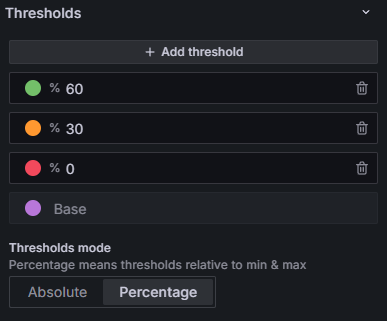
\includegraphics[width=\linewidth, keepaspectratio]{images/thresholds-min-eins.png}
        \caption{Grenzwerte für die KPIs \glqq min. eine Tagebuchseite geöffnet\grqq{} und \glqq min. eine Überschrift aufgeklappt\grqq{}.}
        \label{fig:thresholds-min-eins}
    \end{minipage}
    \hfill
    \begin{minipage}{0.49\textwidth}
        \centering
        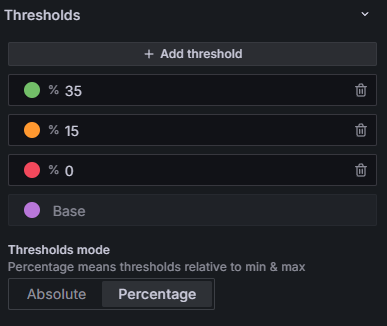
\includegraphics[width=\linewidth, keepaspectratio]{images/thresholds-min-drei.png}
        \caption{Grenzwerte für die KPIs \glqq min. drei Tagebuchseiten geöffnet\grqq{} und \glqq min. drei Überschriften aufgeklappt\grqq{}.}
        \label{fig:thresholds-min-drei}
    \end{minipage}
\end{figure}

Die unterschiedlichen Thresholds verdeutlichen, dass für die beiden Arten von KPIs unterschiedliche Maßstäbe für den Erfolg gelten. Da die Wahrscheinlichkeit, dass Nutzer eine Aktion dreimal ausführen, geringer ist als bei einer einmaligen Ausführung.

Die KPIs zu den Überschriften verwenden das in Listing~\ref{lst:headingsevent} gezeigte \texttt{expand}-Event. Die Tabellen \texttt{log\textunderscore visit} und \texttt{log\textunderscore link\textunderscore visit\textunderscore action} werden hierbei ebenso verknpüft, um die Events mit dem Namen \texttt{expand} zu filtern. Dadurch, dass am Ende der Abfrage nach der Visit-ID für die Sessions gruppiert wird, wird sichergestellt, dass jeder Besuch nur einmal gezählt wird, unabhängig davon, wie oft die Aktion innerhalb eines Besuchs ausgelöst wurde. 



\subsection{Analyse einer Nutzersitzung}

\subsection{Herausforderungen}